\RequirePackage[l2tabu, orthodox]{nag}
% 包含beamer宏包
\documentclass[t, xcolor=svgnames]{ctexbeamer}

% 载入需要的宏包
% 加载宏包
%===================注意======================%
% 在调用beamer.cls宏包后,以下宏包将自动调用,
% 不应单独调用这些宏包,以免发生冲突
% amsfonts, amsmath, amssymb, amsthm, 
% enumerate, geometry, graphics, graphicx, 
% hyperref, url, 
% ifpdf, keyval, xcolor, xxcolor
% =============================================%
% TiKZ绘图宏包
\usepackage{tikz}

% 绘制内存结构图
\usepackage{bytefield}

% 编排代码
\usepackage{minted}

% 绘制UML图
\usepackage{pgf-umlcd}

% 用TiKZ绘制流程图
% 自定义宏包,参见:https://github.com/registor/tikz-flowchart
\usepackage{tikz-flowchart}

%%% Local Variables: 
%%% mode: latex
%%% TeX-master: "../main.tex"
%%% End:


% 进行必要的设置
% ====================================================================================
% bytefield绘图设置
% 调整表格的垂直对齐方式
\newcommand{\descbox}[1]{\parbox[c][0.7\baselineskip]{0.95\width}{%
\raggedright #1\vfill}}
% 用于绘制无标记内存图中一个内存块的命令,其开始地址在底部,结束地址在顶部(基于bytefield宏包)
% 语法:
% \memsec{结束地址}{开始地址}{以行为单位的高度}{盒子中的文字}
\newcommand*\istempaddr[1]{\IfStrEq{}{#1}{}{0X#1}}
\newcommand{\memsec}[4]{%
  % 定义memsection的高度
  %
  %\tiny
  \bytefieldsetup{bitheight=#3\baselineskip}%
  \bitbox[]{5}{%    
    \tiny \texttt{\istempaddr{#1}}%0X#1}% 结束地址
    \\
    % 留出空白
    \vspace{#3\baselineskip}
    \vspace{-1.6\baselineskip}
    \vspace{-#3pt}
    \tiny \texttt{\istempaddr{#2}}%0X#2}% 开始地址
  }%
  \bitbox{4}{\tiny \texttt{#4}}% 盒子里的内容 %\vspace{-0.9\baselineskip}
}

% 定义绘制有标记内存的命令(基于bytefield宏包)
% 创建计算机内存映像的自定义命令,
% 起始地址位于低部,结束地址位于顶部
% 语法:
% \memsection[标记符号]{结束地址}{起始地址}{内存单元高度}{内存单元中的内容}
% 其中标记符号为可选项,可以是任何符合LaTeX语法的内容
\newcommand{\memseclab}[5][]{
  %\tiny
  \bytefieldsetup{bitheight=#4\baselineskip} % 内存单元的高度
  \bitbox[]{10}{%标记符号及地址盒子,参数为总宽度
    \raggedleft%右对齐
    \texttt{\tiny\istempaddr{#2}}% 结束地址
    \\%换行
    % 设置结束地址与起始地址之间的空白
    \vspace{#4\baselineskip}
    \vspace{-1.5\baselineskip}
    \vspace{-#4pt} % 
    {\tiny\texttt{#1}}%\hspace{1em}
    \texttt{\tiny\istempaddr{#3}}% 起始地址
  }~
  \bitbox{4}{\tiny \texttt{#5}} % 内存单元盒子
}

% 自定义垂直省略号
\makeatletter
\DeclareRobustCommand{\rvdots}{%
  \vbox{
    \baselineskip4\p@\lineskiplimit\z@
    \kern-\p@
    \hbox{.}\hbox{.}\hbox{.}
  }}
\makeatother
% ====================================================================================

% ====================================================================================
% 重定义强调字体的代码,解决默认强调字体是italic,此时中文会用楷体代替,
% 在此设置为加粗,注意需要使用etoolbox宏包
\makeatletter
\let\origemph\emph
\newcommand*\emphfont{\normalfont\bfseries}
\DeclareTextFontCommand\@textemph{\emphfont}
\newcommand\textem[1]{%
  \ifdefstrequal{\f@series}{\bfdefault}
    {\@textemph{\CTEXunderline{#1}}}
    {\@textemph{#1}}%
}
\RenewDocumentCommand\emph{s o m}{%
  \IfBooleanTF{#1}
    {\textem{#3}}
    {\IfNoValueTF{#2}
      {\textem{#3}\index{#3}}
      {\textem{#3}\index{#2}}%
     }%
}
\makeatother   
% ====================================================================================

% 代码显示模式设置(基于minted宏包)
% ====================================================================================
\usemintedstyle{default}  %codeblocks模式

% 定义排版C语言代码命令
\setminted{fontsize=\tiny, breaklines=true,
  breakautoindent=false}
\newmintinline{c}{fontsize=\normalsize, autogobble}
\newmintinline[cinlinett]{c}{fontsize=\normalsize, escapeinside=||, autogobble}
\newmintinline[cinttscr]{c}{fontsize=\scriptsize, escapeinside=||, autogobble}
\newmintinline[cinttfts]{c}{fontsize=\footnotesize, escapeinside=||, autogobble}
\newmintinline[cintttny]{c}{fontsize=\tiny, escapeinside=||, autogobble}
\newmintinline[cinttlrg]{c}{fontsize=\large, escapeinside=||, autogobble}
\newminted{c}{frame=lines, autogobble}
\newminted[ctt]{c}{mathescape,frame=lines,escapeinside=||, autogobble}
\newmintedfile{c}{frame=lines}%linenos=true,
\newmintedfile[cfilett]{c}{frame=lines,escapeinside=||}%linenos=true,
\newmintedfile[cfttscr]{c}{fontsize = \scriptsize, frame=lines,escapeinside=||}%linenos=true,
\newmintedfile[cfiletikz]{c}{frame=lines}%linenos=true,
% ====================================================================================

% TikZ宏包扩展
% ====================================================================================
\usetikzlibrary{graphs}
\usetikzlibrary{mindmap,trees}
\tikzset{every concept/.style={minimum size=1cm, text width=1.5cm}}
\usetikzlibrary{shapes,arrows,chains}
\usetikzlibrary{positioning}
\usetikzlibrary{calc}
\usetikzlibrary{arrows.meta}
\usetikzlibrary{decorations.pathreplacing}
\usetikzlibrary{tikzmark}
\usetikzlibrary{shapes.geometric}
\usetikzlibrary{decorations.text}
\usetikzlibrary{matrix}
\usetikzlibrary{backgrounds}
% ====================================================================================

% %%%%%%%%%% 绘制流程图时TiKz宏包的设置 %%%%%%%%
% 作者: Brent Longborough
% URL:http://www.texample.net/tikz/examples/author/brent-longborough/
% ====================================================================================
% 定义颜色名称
\colorlet{lcfree}{green}
\colorlet{lcnorm}{blue}
\colorlet{lccong}{red}
% 设置一个用于调试的标记符号图层,注意确保这一图层位于顶层
\pgfdeclarelayer{marx}
\pgfsetlayers{main,marx}

% 标记坐标点的宏命令(指定使用的坐标名称)
% 可以通过交替注释以下两个宏命令定义,以打开和关闭调试功能。
\providecommand{\cmark}[2][]{%
  \begin{pgfonlayer}{marx}
    \node [nmark] at (c#2#1) {#2};
  \end{pgfonlayer}{marx}
  } 
%\providecommand{\cmark}[2][]{\relax} 
% -------------------------------------------------
\tikzset{
  start chain = going below,    % 自顶向下绘制
  node distance = 6mm and 60mm, % 结点距离的全局设置
  every join/.style = {norm},   % 默认的结点连线样式
  %every picture/.style={thick},
  base/.style = {draw, thick, on chain, on grid, align=center, minimum height=2ex},%基本样式
  proc/.style={base, rectangle, text width=4em, fill=orange!10},%处理框样式
  test/.style={base, diamond, aspect=2.5, text width=3em, fill=green!30},%判断框样式
  io/.style={base, trapezium, trapezium left angle=70, trapezium right
    angle=110, text width=6em,  fill=blue!30},%输入/输出框样式
  term/.style={proc, rounded corners, text width=3em, fill=red!30},%开始结束框样式
  % 流程连接点样式
  connector/.style = {draw,circle,node distance=3cm,fill=yellow!20},
  % coord结点样式用于绘制连接线的角点
  coord/.style={coordinate, on chain, on grid, node distance=6mm and 25mm},
  % nmark结点样式用于绘制调试中的坐标标记
  nmark/.style={draw, cyan, circle, font={\sffamily\bfseries}},
  % 不相交的两个交汇路径的连接样式
  connect/.style args={(#1) to (#2) over (#3) by #4}{
        insert path={
            let \p1=($(#1)-(#3)$), \n1={veclen(\x1,\y1)}, 
            \n2={atan2(\y1,\x1)}, \n3={abs(#4)}, \n4={#4>0 ?-180:180}  in 
            (#1) -- ($(#1)!\n1-\n3!(#3)$) 
            arc (\n2:\n2+\n4:\n3) -- (#2)
        }
    }, 
  % -------------------------------------------------
  % 流程图中无箭头连线样式
  lnorm/.style={thick, draw, lcnorm},
  lfree/.style={thick, draw, lcfree},
  lcong/.style={thick, draw, lccong},
  % 流程图中流程线汇聚实心样式
  dotnorm/.style={draw, fill = lcnorm, lcnorm},
  dotfree/.style={draw, fill = lcfree, lcfree},
  dotcong/.style={draw, fill = lccong, lccong},
   % 流程图中流程线汇聚空心样式
  cdotnorm/.style={draw, lcnorm},
  cdotfree/.style={draw, lcfree},
  cdotcong/.style={draw, lccong},
  % 流程图中有箭头连线样式
  norm/.style={thick, ->, >=stealth, draw, lcnorm},
  free/.style={thick, ->, >=stealth, draw, lcfree},
  cong/.style={thick, ->, >=stealth, draw, lccong},
  it/.style={font={\small\itshape}},
}
% ====================================================================================

% 设置动画显示样式
% ====================================================================================
\tikzset{
  invisible/.style={opacity=0},
  visible on/.style={alt={#1{}{invisible}}},
  alt/.code args={<#1>#2#3}{%
    \alt<#1>{\pgfkeysalso{#2}}{\pgfkeysalso{#3}} % \pgfkeysalso doesn't change the path
  },
}
% ====================================================================================

%%%%%%%%%% 绘制链表数据结构需要的命令TiKz%%%%%%%%
% ====================================================================================
\usetikzlibrary{shapes,arrows,calc}
\newcommand{\data}{data \nodepart{second} \phantom{null}}

\tikzstyle{ptr}  = [draw, -latex', blue]
\tikzstyle{head} = [rectangle, draw, text height=3mm, text width=3mm, text centered, node distance=3cm, inner sep=0pt]
\tikzstyle{data} = [rectangle split, rectangle split parts=2, draw, text centered, minimum height=3em]
% ====================================================================================

% 改变脚注的符号
% ====================================================================================
\setbeamerfont{footnote}{size=\zihao{7}} % 改变脚注字号
\makeatletter
\def\@fnsymbol#1{\ensuremath{\ifcase#1\or *\or \dagger\or \ddagger\or
   \mathsection\or \mathparagraph\or \|\or **\or \dagger\dagger
   \or \ddagger\ddagger \else\@ctrerr\fi}}
\makeatother
\renewcommand{\thefootnote}{\fnsymbol{footnote}}
% ====================================================================================

% 定义C语言中的专有名词命令
% ====================================================================================
\newcommand{\cb}{\texttt{Code::Blocks}}
\newcommand{\mww}{\texttt{MinGW-w64}}
\newcommand{\mfile}{\qtmark{\texttt{Makefile}}}
\newcommand{\vs}{\texttt{Visual Studio}}
\newcommand{\gcc}{\texttt{gcc}}
\newcommand{\db}{\texttt{DEBUG}}
\newcommand{\dbger}{\texttt{Debugger}}
\newcommand{\gdb}{\texttt{gdb}调试器}
\newcommand{\cdb}{\texttt{cdb}调试器}
\newcommand{\gdbcmd}{\texttt{(gdb)}}
\newcommand{\scf}{\cinline[fontsize = \scriptsize]{scanf()}}
\newcommand{\ptf}{\cinline{printf()}}
\newcommand{\rn}{\cinline{'\n'}}
\newcommand{\cch}[1]{\cinline{'#1'}}
\newcommand{\lumos}{Linux、Unix、Mac OS}
\newcommand{\win}{Windows}
\newcommand{\unix}{UNIX}
\newcommand{\lnx}{Linux}

\newcommand{\cl}{{C语言}}
\newcommand{\nint}{{\cinline{int}}}
\newcommand{\flt}{{\cinline{float}}}
\newcommand{\snint}{{\cinline{short int}}}
\newcommand{\lint}{{\cinline{long int}}}
\newcommand{\llint}{{\cinline{long long int}}}
\newcommand{\ldb}{{\cinline{long double}}}
\newcommand{\sch}{{\cinline{signed char}}}
\newcommand{\sint}{{\cinline{signed int}}}
\newcommand{\ssint}{{\cinline{signed short int}}}
\newcommand{\slint}{{\cinline{signed long int}}}
\newcommand{\sllint}{{\cinline{signed long long int}}}
\newcommand{\usch}{{\cinline{unsigned char}}}
\newcommand{\usint}{{\cinline{unsigned int}}}
\newcommand{\ussint}{{\cinline{unsigned short int}}}
\newcommand{\uslint}{{\cinline{unsigned long int}}}
\newcommand{\usllint}{{\cinline{unsigned long long int}}}

% 路径设置
% ====================================================================================
\graphicspath{{figure/}}%图片所在的目录
% ====================================================================================


%%% Local Variables: 
%%% mode: latex
%%% TeX-master: "../main.tex"
%%% End: 


\begin{document}

\begin{frame}[fragile] % minted宏包排版代码,需要[fragile]参数
  \begin{itemize}
  \item 应用实例
  \end{itemize}
  \begin{center}
    \begin{tikzpicture}[font=\tiny]
      \tikzset{ coord/.style={coordinate} }
      \umlnote[text width=0.65\textwidth](code1) at (0, 0)
      {
        \begin{ccode}
          int iValue;             /*整型类型*/
          int * piValue;         /*整型地址类型*/
          
          piValue = &iValue;  /*将iValue的地址赋与指针*/
          iValue = 65;            /*给iValue赋值*/
          *piValue = 97;         /*给piValue指向的内存赋值*/
        \end{ccode}
      };                  

      \node[below = 0.8 of code1, xshift = -2.5cm] (mem01) {
        \begin{bytefield}[rightcurlyspace=0pt]{4}%rightcurly=.,{24}
          \begin{rightwordgroup}{piValue}
            \memsec{FFFF E317}{FFFF E310}{8}{0000 7FFF\\ FFFF E30C}
          \end{rightwordgroup}\\
          \begin{rightwordgroup}{iValue}
            \memsec{FFFF E30F}{FFFF E30C}{4}{0000 0041}
          \end{rightwordgroup}
        \end{bytefield}
      };
      \node[below = 0.1 of mem01] (note01) {\cintttny{iValue = 65}};

      % 计算绘图坐标
      \path let \p1=(mem01) in
      coordinate (org) at (\x1, \y1)
      coordinate (ovBL1) at ($(org) + (-1.75, -1.32)$)
      coordinate (ovUR1) at ($(ovBL1) + (1.35, 0.25)$)
      coordinate (ovTL1) at ($(ovBL1) + (0.0, 0.25)$)
      coordinate (ovML1) at ($(ovTL1)!0.5!(ovBL1)$)
      coordinate (ovMLO1) at ($(ovML1) + (-0.2, 0.0)$)
      
      coordinate (ovBL2) at ($(ovBL1) + (1.35, 0.89)$)
      coordinate (ovUR2) at ($(ovBL2) + (1.12, 1.69)$)
      coordinate (ovTL2) at ($(ovBL2) + (0.0, 1.69)$)
      coordinate (ovML2) at ($(ovTL2)!0.5!(ovBL2)$)
      coordinate (ovMLO2) at ($(ovML2) + (-1.55, 0.0)$)
      coordinate (ovVN1) at ($(ovML2) + (2.2, 0.0)$)
      coordinate (ovVN2) at ($(ovVN1) + (-0.15, -1.25)$)
      coordinate (ovVN2T) at ($(ovVN2) + (0.1, 0.0)$)
      coordinate (ovDAT) at ($(ovVN2T) + (0.0, -0.8)$)
      ;

      \node[draw] (dat) at (ovDAT) {65};
      
      \draw[red,thick,fill=green!35, fill opacity=0.3](ovBL1) rectangle
      (ovUR1);
      \draw[blue,thick,fill=red!35, fill opacity=0.3](ovBL2) rectangle
      (ovUR2);

      \draw[-{Stealth[scale=1.0]}, red, thick] (ovML1) -- (ovMLO1) --
      (ovMLO2)--node[above,black]{取地址}(ovML2);
      
      \draw[-{Stealth[scale=1.0]}, blue, thick] (ovVN1) to [out =
      -45, in = 45] node[right,align=left,yshift=0.0cm,black]{指
        \\向}(ovVN2);
      
      \draw[-{Stealth[scale=1.0]}, blue, thick] (dat.north) to [out =
      90, in = -90] node[right,align=left,yshift=0.0cm,black]{赋
        值}(ovVN2T);      

      \node[right = 0.8 of mem01] (mem02) {
        \begin{bytefield}[rightcurlyspace=0pt]{4}%rightcurly=.,{24}
          \begin{rightwordgroup}{piValue}
            \memsec{FFFF E317}{FFFF E310}{8}{0000 7FFF\\ FFFF E30C}
          \end{rightwordgroup}\\
          \begin{rightwordgroup}{iValue}
            \memsec{FFFF E30F}{FFFF E30C}{4}{0000 0061}
          \end{rightwordgroup}
        \end{bytefield}
      };
      \node[below = 0.1 of mem02] (note02) {\cintttny{*piValue = 97}};

      % 计算绘图坐标
      \path let \p1=(mem02) in
      coordinate (org) at (\x1, \y1)
      coordinate (ovBL1) at ($(org) + (-1.75, -1.32)$)
      coordinate (ovUR1) at ($(ovBL1) + (1.35, 0.25)$)
      coordinate (ovTL1) at ($(ovBL1) + (0.0, 0.25)$)
      coordinate (ovML1) at ($(ovTL1)!0.5!(ovBL1)$)
      coordinate (ovMLO1) at ($(ovML1) + (-0.2, 0.0)$)
      
      coordinate (ovBL2) at ($(ovBL1) + (1.35, 0.89)$)
      coordinate (ovUR2) at ($(ovBL2) + (1.12, 1.69)$)
      coordinate (ovTL2) at ($(ovBL2) + (0.0, 1.69)$)
      coordinate (ovML2) at ($(ovTL2)!0.5!(ovBL2)$)
      coordinate (ovMLO2) at ($(ovML2) + (-1.55, 0.0)$)
      coordinate (ovVN1) at ($(ovML2) + (2.2, 0.0)$)
      coordinate (ovVN2) at ($(ovVN1) + (-0.15, -1.25)$)
      coordinate (ovPT) at ($(ovVN1) + (0.0, 0.8)$)
      ;

      \node[draw] (dat) at (ovPT) {97};

      \draw[red,thick,fill=green!35, fill opacity=0.3](ovBL1) rectangle
      (ovUR1);
      \draw[blue,thick,fill=red!35, fill opacity=0.3](ovBL2) rectangle
      (ovUR2);

      \draw[-{Stealth[scale=1.0]}, red, thick] (ovML1) -- (ovMLO1) --
      (ovMLO2)--node[above,black]{取地址}(ovML2);
      
      \draw[-{Stealth[scale=1.0]}, blue, thick] (ovVN1) to [out =
      -45, in = 45] node[right,align=left,yshift=0.0cm,black]{指
        \\向}(ovVN2);

      \draw[-{Stealth[scale=1.0]}, blue, thick] (dat) to [out =
      -90, in = 90] node[right,align=left,xshift=0.3cm,yshift=0.2cm,black]{地\\
        址}(ovVN1);
    \end{tikzpicture}\let\thefootnote\relax\footnote[frame]{此处省略64位地址的前4个字节0X0000 7FFF。}
  \end{center} 
\end{frame}

\begin{frame}[fragile] % minted宏包排版代码,需要[fragile]参数
  \begin{itemize}
  \item 同种数据类型的数据集合
    \begin{itemize}
    \item 指针索引
    \end{itemize}
  \end{itemize}
  \begin{center}
    \begin{tikzpicture}[font=\tiny]
      \tikzset{ coord/.style={coordinate} }
      \umlnote[text width=0.75\textwidth](code1) at(0, 0)
      {
        \cfile{codes/main.c}
      };

      \node[below = 0.02 of code1,xshift = 0.05cm] (mem01) {
        \begin{bytefield}[rightcurly=., rightcurlyspace=0pt]{4}
          \memsec{}{}{2}{\rvdots}\\
          \begin{rightwordgroup}{fCGrade[89]}
            \memsec{FFFF E317}{FFFF E314}{2}{}
          \end{rightwordgroup}\\
          \begin{rightwordgroup}{\rvdots}
            \memsec{FFFF E313}{FFFF E1E0}{2}{\rvdots}
          \end{rightwordgroup}\\
          \begin{rightwordgroup}{fCGrade[11]}
            \memsec{FFFF E1DF}{FFFF E1DC}{2}{80.0}
          \end{rightwordgroup}\\
          \begin{rightwordgroup}{\rvdots}
            \memsec{FFFF E1DB}{FFFF E1C4}{2}{\rvdots}
          \end{rightwordgroup}\\
          \begin{rightwordgroup}{fCGrade[4]}
            \memsec{FFFF E1C3}{FFFF E1C0}{2}{87.0}
          \end{rightwordgroup}\\
          \begin{rightwordgroup}{\rvdots}
            \memsec{FFFF E1BF}{FFFF E1B4}{2}{\rvdots}
          \end{rightwordgroup}\\
          \begin{rightwordgroup}{fCGrade[0]}
            \memsec{FFFF E1B3}{FFFF E1B0}{2}{80.0}
          \end{rightwordgroup}\\
          \begin{rightwordgroup}{pArray}
            \memsec{FFFF E1AF}{FFFF E1AC}{2}{\alert{FFFF E1B0}}
          \end{rightwordgroup}\\
          \memsec{}{}{2}{\rvdots}
        \end{bytefield}
      };

      % 计算绘图坐标
      \path let \p1=(mem01) in coordinate (org) at (\x1, \y1)
      coordinate (ovBL1) at ($(org) + (-1.84, -1.28)$)%
      coordinate (ovUR1) at ($(ovBL1) + (1.32, 0.20)$)%
      coordinate (ovTL1) at ($(ovBL1) + (0.0, 0.20)$)%
      coordinate (ovML1) at ($(ovTL1)!0.5!(ovBL1)$)%
      coordinate (ovMLO1) at ($(ovML1) + (-0.2, 0.0)$)%
      
      coordinate (ovBL2) at ($(ovBL1) + (1.35, -0.4)$)%
      coordinate (ovUR2) at ($(ovBL2) + (1.12, 0.41)$)%
      coordinate (ovTL2) at ($(ovBL2) + (0.0, 0.41)$)%
      coordinate (ovML2) at ($(ovTL2)!0.5!(ovBL2)$)%
      coordinate (ovMLO2) at ($(ovML2) + (-1.55, 0.0)$)%

      coordinate (ovVN0) at ($(ovML2) + (1.9, 0.0)$)%
      coordinate (ovVN1) at ($(ovVN0) + (0.5, 0.0)$)%
      coordinate (ovVN2) at ($(ovVN1) + (-0.15, 0.4)$)%
      coordinate (ovVN3) at ($(ovVN1) + (-0.05, 2.15)$)%
      coordinate (ovVN4) at ($(ovVN1) + (-0.15, 1.35)$) ;

      \draw[-{Stealth[scale=1.0]}, red, thick] (ovML1) -- (ovMLO1) --
      node[left,align=right,black](getadd){取\\地\\址}(ovMLO2)--(ovML2);

      \node[left = 0.05 of getadd] (getaddnote) {\cintttny{pArray = fCGrade}};

      \draw[red,thick,fill=green!35, fill opacity=0.3](ovBL1)
      rectangle (ovUR1);
      \draw[blue,thick,fill=red!35, fill opacity=0.3](ovBL2) rectangle
      (ovUR2);
      
      \draw[-{Stealth[scale=1.0]}, blue, thick] (ovVN0) to [out = 0,
      in = 180]node[below, xshift = 0.05cm, yshift = 0.1cm,
      black](pt01){指向}(ovVN1) to [out = 0, in = -45]
      node[fill=green!25, right,xshift = 0.25cm, xshift = 0.3cm, yshift = 0.25cm,
      black] {\cintttny{*pArray =80.0}}(ovVN2);

      \draw[-{Stealth[scale=1.0]}, blue, thick] (ovVN1) to [out = 0,
      in = -45] node[fill = green!25,right,xshift = -0.15cm,yshift =
      1.3cm, black] {\cintttny{*(pArray + 5 + 6) = 80.0}}(ovVN3);
          
      \draw[-{Stealth[scale=1.0]}, blue, thick] (ovVN1) to [out = 0,
      in = -45] node[fill = green!25, right, xshift = 0.25cm, yshift =
      0.7cm, black] {\cintttny{pArray[4] = 87.0}}(ovVN4);
    \end{tikzpicture}
  \end{center}
\end{frame}

\begin{frame}[fragile] % minted宏包排版代码,需要[fragile]参数
  \begin{itemize}
  \item 冒泡排序(\alert{减少循环次数})
  \end{itemize} 
  \begin{center}
    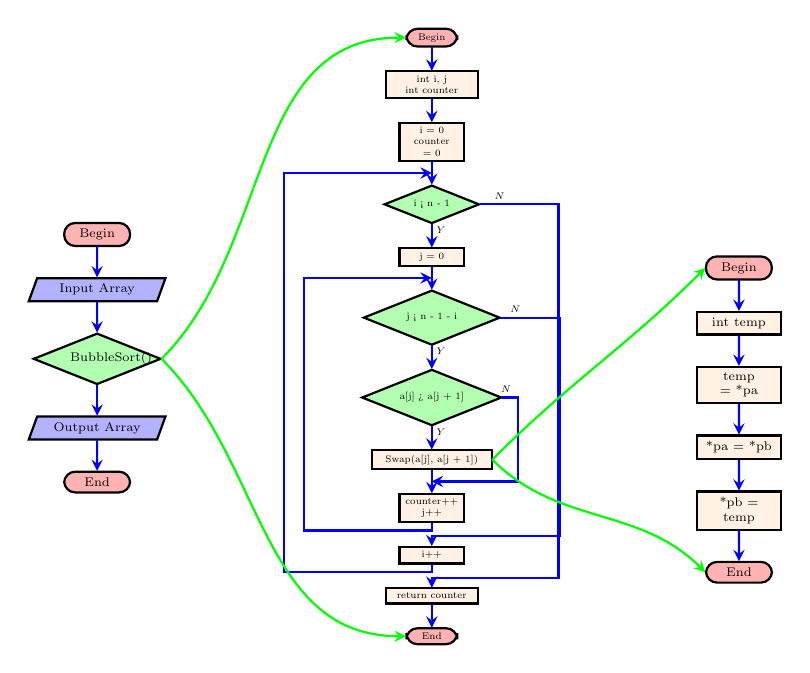
\begin{tikzpicture}[font=\scriptsize]
      \tikzset{ coord/.style={coordinate} }
      \begin{scope}[scale = 0.65, every node/.append style = {transform shape}]
        % 布置结点单元
        \node [term] (st1) at (0, 0) {Begin};
        \node [io, join] (i1) {Input Array};
        \node [test, join] (t0) {\alert{BubbleSort()}};
        \node [io, join] (o1) {Output Array};
        \node [term, join] (end1) {End};
      \end{scope}
      \begin{scope}[scale = 0.5, every node/.append style = {transform
          shape}]%transform canvas = {scale=0.8}, overlay
        % 布置结点单元
        \node [term, right =8.5 of st1, shift={(0.0cm, 5.0cm)}] (st2) {Begin};
        \node [proc, text width = 6em, join] (p1) {\cinttscr{int i, j}\\\cinttscr{int counter}};
        \node [proc, join] (p2) {\cinttscr{i = 0}\\\cinttscr{counter = 0}};
        \node [test, join] (t1) {\cinttscr{i < n - 1}};
        \node [proc] (p3) {\cinttscr{j = 0}};
        \node [test, text width = 6em, join] (t2) {\cinttscr{j < n - 1 - i}};
        \node [test, text width = 6em] (t3) {\cinttscr{a[j] > a[j + 1]}};
        \node [proc, text width = 8em] (p4) {\cinttscr{Swap(a[j], a[j + 1])}};
        \node [proc, join] (p5) {\cinttscr{counter++}\\\cinttscr{j++}};
        \node [proc] (p6) {\cinttscr{i++}};
        \node [proc, text width = 6em] (p7) {\cinttscr{return counter}};
        \node [term, join] (end2) {End};%, below = 1.6 of p3

        % 布置用于连接的坐标结点,同时为其布置调试标记点。
        \node [coord] (c1) at ($(p2.south)!0.5!(t1.north)$)  {};% \cmark{1}
        \node [coord] (c2) at ($(p3.south)!0.5!(t2.north)$)  {};% \cmark{2}
        \node [coord] (c3) at ($(p4.south)!0.5!(p5.north)$)  {};% \cmark{3}
        \node [coord, below = 0.2 of p5] (c4)  {};% \cmark{4}
        \node [coord, above = 0.25 of p6] (c5) {}; % \cmark{5}
        \node [coord, below = 0.2 of p6] (c6)  {};% \cmark{6}
        \node [coord, above = 0.25 of p7] (c7)  {};% \cmark{7}
        \node [coord, right = 2.0 of t1] (c8) {}; % \cmark{8}
        \node [coord, right = 1.5 of t2] (c9) {}; % \cmark{9}
        \node [coord, right = 0.4 of t3] (c10) {}; % \cmark{10}
        \node [coord, left = 1.5 of t2] (ct1) {}; % \cmark{t1}
        \node [coord, left = 2.0 of t2] (ct2) {}; % \cmark{t2}
        \node [coord] (c11) at (c6 -| ct2)  {};% \cmark{11}
        \node [coord] (c12) at (c4 -| ct1)  {};% \cmark{12}
        

        % 判断框连线,每次绘制时,先绘制一个带有一个固定
        % 位置标注的路径(path),然后再绘制箭头本身(arrow)。
        \path (t1.south) -- node [near start, right] {$Y$} (p3.north);
        \draw [norm] (t1.south) -- (p3.north);
        \path (t1.east) -- node [near start, above] {$N$} (c8);
        \draw [norm] (t1.east) -- (c8) |- (c7) -- (p7.north);
        
        \path (t2.south) -- node [near start, right] {$Y$} (t3.north);
        \draw [norm] (t2.south) -- (t3.north);
        \path (t2.east) -- node [near start, above] {$N$} (c9);
        \draw [norm] (t2.east) -- (c9) |- (c5) -- (p6.north);
        
        \path (t3.south) -- node [near start, right] {$Y$} (p4.north);
        \draw [norm] (t3.south) -- (p4.north);
        \path (t3.east) -- node [near start, above] {$N$} (c10);
        \draw [norm] (t3.east) -- (c10) |- (c3);

        % 其它连线
        \draw [norm](p5.south) |- (c12) |- (c2);
        \draw [norm](p6.south) |- (c11) |- (c1);
      \end{scope}
      \begin{scope}[scale = 0.65, every node/.append style = {transform
          shape}]%transform canvas = {scale=0.8}, overlay
        % 布置结点单元
        \node [term,  right =6.0 of st2, shift={(0.0cm, -4.5cm)}] (st3) {Begin};
        \node [proc, join] (p7) {int temp};
        \node [proc, join] (p8) {temp = *pa};
        \node [proc, join] (p9) {*pa = *pb};
        \node [proc, join] (p10) {*pb = temp};        
        \node [term, join] (end3) {End};
      \end{scope}
      % 绘制Sort函数调用关系
      \draw [free] (t0.east) to [out = 45, in = 180] (st2.west);
      \draw [free] (t0.east) to [out = -45, in = 180] (end2.west);
      % 绘制Swap函数调用关系
      \draw [free] (p4.east) to [out = 45, in = -135] (st3.west);
      \draw [free] (p4.east) to [out = -45, in = 135] (end3.west);
      % % 绘制函数调用关系
      % \draw [free] (t0.east) to [out = 45, in = -175] (st2.west);
      % \draw [free] (t0.east) to [out = -45, in = 175] (end2.west);
    \end{tikzpicture}
  \end{center}
\end{frame}


\begin{frame}[fragile] % minted宏包排版代码,需要[fragile]参数
  \begin{itemize}
  \item 动态数组作函数参数   
  \end{itemize}
  \begin{center}
    \begin{tikzpicture}[font=\tiny]
      \umlnote[scale = 0.8, text width=0.55\textwidth](code1) at(0, 0)
      {
        \cfile{codes/memdiagram.c} % 载入C代码文件,用minted排版
      };

      \node[scale = 0.95, right = 0.5 of code1, shift={(-1.8cm, 0.0cm)}] (mem01) {
        % 用bytefield宏包绘制内存结构图
        \begin{bytefield}[leftcurlyspace=34pt,
          rightcurlyspace=0pt]{4}
          \memsec{}{}{2}{\rvdots}\\
          \begin{rightwordgroup}{栈}
            \begin{leftwordgroup}{pa:main}
              \memsec{}{FFFF E180}{2}{$\ldots$}
            \end{leftwordgroup}\\
            \memsec{}{}{2}{\rvdots}\\
            \begin{leftwordgroup}{p:Traversal}
              \memsec{}{FFFF E158}{2}{$\ldots$}
            \end{leftwordgroup}\\
            \memsec{}{}{2}{\rvdots}\\
            \begin{leftwordgroup}{pa:Traversal}
              \memsec{}{FFFF E148}{2}{$\ldots$}
            \end{leftwordgroup}\\
            \memsec{}{}{2}{\rvdots}\\
            \begin{leftwordgroup}{pf:Traversal}
              \memsec{}{FFFF E138}{2}{$\ldots$}
            \end{leftwordgroup}\\
            \memsec{}{}{2}{\rvdots}\\
            \begin{leftwordgroup}{pData:I/Oput}
              \memsec{}{FFFF E118}{2}{$\ldots$}
            \end{leftwordgroup}
          \end{rightwordgroup}\\
          \memsec{}{}{2}{\rvdots}\\
          \begin{rightwordgroup}{堆}            
            \memsec{}{}{1}{$\ldots$}\\%
            \memsec{}{}{1}{$\ldots$}\\%
            \memsec{}{}{1}{$\ldots$}\\%
            \memsec{}{}{1}{$\ldots$}\\%
            \memsec{}{}{1}{$\ldots$}\\%
            \memsec{}{}{1}{$\ldots$}\\%
            \memsec{}{0060 3430}{1}{$\ldots$}
          \end{rightwordgroup}\\
          \memsec{}{}{2}{\rvdots}\\
          \begin{rightwordgroup}{代码段}
            \memsec{}{0040 0935}{2}{Output()}\\%
            \memsec{}{0040 0910}{2}{Input()}
          \end{rightwordgroup}\\
          \memsec{}{}{2}{\rvdots}
        \end{bytefield}
      };
      
      \def\clh{1.1ex}; % 一行代码高度
      \def\clw{3.35em}; % 一行代码宽度
      \def\stpos{-5.65em} % 标记框起始x轴位置
      \path let \p1=(code1) in coordinate (org1) at (\x1, \y1)
      % pa指针声明代码坐标
      coordinate (ovBL10) at ($(org1) + (\stpos, 11.10 * \clh)$)%左下角坐标
      coordinate (ovUR10) at ($(ovBL10) + (\clw, \clh)$)%右上角坐标
      coordinate (ovCD10) at ($(ovBL10)!0.5!(ovUR10)$)%中心点坐标
      coordinate (ovCR10) at (ovUR10|-ovCD10)%右边线中点坐标
      % 通过pa指针分配内存代码坐标
      coordinate (ovBL11) at ($(ovBL10) + (0.0, -3.08 * \clh)$)%左下角坐标
      coordinate (ovUR11) at ($(ovBL11) + (2.35 * \clw, \clh)$)%右上角坐标
      coordinate (ovCD11) at ($(ovBL11)!0.5!(ovUR11)$)%中心点坐标
      coordinate (ovCR11) at (ovUR11|-ovCD11)%右边线中点坐标
      % 遍历函数第1次调用pa实参代码坐标
      coordinate (ovBL12) at ($(ovBL10) + (0.7 * \clw, -5.18 * \clh)$)%左下角坐标
      coordinate (ovUR12) at ($(ovBL12) + (0.17 * \clw, \clh)$)%右上角坐标
      coordinate (ovCD12) at ($(ovBL12)!0.5!(ovUR12)$)%中心点坐标
      coordinate (ovCR12) at (ovUR12|-ovCD12)%右边线中点坐标
      % 遍历函数第1次调用Input实参代码坐标
      coordinate (ovBL13) at ($(ovBL12) + (0.44 * \clw, 0.0)$)%左下角坐标
      coordinate (ovUR13) at ($(ovBL13) + (0.37 * \clw, \clh)$)%右上角坐标
      coordinate (ovCD13) at ($(ovBL13)!0.5!(ovUR13)$)%中心点坐标
      coordinate (ovCR13) at (ovUR13|-ovCD13)%右边线中点坐标
       % 遍历函数第2次调用pa实参代码坐标
      coordinate (ovBL14) at ($(ovBL12) + (0.0, -2.10 * \clh)$)%左下角坐标
      coordinate (ovUR14) at ($(ovBL14) + (0.17 * \clw, \clh)$)%右上角坐标
      coordinate (ovCD14) at ($(ovBL14)!0.5!(ovUR14)$)%中心点坐标
      coordinate (ovCR14) at (ovUR14|-ovCD14)%右边线中点坐标
      % 遍历函数第2次调用Output实参代码坐标
      coordinate (ovBL15) at ($(ovBL14) + (0.44 * \clw, 0.0)$)%左下角坐标
      coordinate (ovUR15) at ($(ovBL15) + (0.44 * \clw, \clh)$)%右上角坐标
      coordinate (ovCD15) at ($(ovBL15)!0.5!(ovUR15)$)%中心点坐标
      coordinate (ovCR15) at (ovUR15|-ovCD15)%右边线中点坐标
      % free函数调用代码坐标
      coordinate (ovBL16) at ($(ovBL10) + (0.0, -10.40 * \clh)$)%左下角坐标
      coordinate (ovUR16) at ($(ovBL16) + (0.66 * \clw, \clh)$)%右上角坐标
      coordinate (ovCD16) at ($(ovBL16)!0.5!(ovUR16)$)%中心点坐标
      coordinate (ovCR16) at (ovUR16|-ovCD16)%右边线中点坐标
      % NULL空指针操作代码坐标
      coordinate (ovBL17) at ($(ovBL16) + (0.0, -1.10 * \clh)$)%左下角坐标
      coordinate (ovUR17) at ($(ovBL17) + (0.66 * \clw, \clh)$)%右上角坐标
      coordinate (ovCD17) at ($(ovBL17)!0.5!(ovUR17)$)%中心点坐标
      coordinate (ovCR17) at (ovUR17|-ovCD17)%右边线中点坐标
      % Traversal形参pa代码坐标
      coordinate (ovBL18) at ($(ovBL17) + (1.16 * \clw, -3.15 * \clh)$)%左下角坐标
      coordinate (ovUR18) at ($(ovBL18) + (0.17 * \clw, \clh)$)%右上角坐标
      coordinate (ovCD18) at ($(ovBL18)!0.5!(ovUR18)$)%中心点坐标
      coordinate (ovCR18) at (ovUR18|-ovCD18)%右边线中点坐标
      % Traversal形参pf代码坐标
      coordinate (ovBL19) at ($(ovBL18) + (1.15 * \clw, 0.0)$)%左下角坐标
      coordinate (ovUR19) at ($(ovBL19) + (0.16 * \clw, \clh)$)%右上角坐标
      coordinate (ovCD19) at ($(ovBL19)!0.5!(ovUR19)$)%中心点坐标
      coordinate (ovCR19) at (ovUR19|-ovCD19)%右边线中点坐标
      % 遍历函数内p指针声明代码坐标
      coordinate (ovBL1a1) at ($(ovBL17) + (0.00, -5.20 * \clh)$)%左下角坐标
      coordinate (ovUR1a1) at ($(ovBL1a1) + (0.50 * \clw, \clh)$)%右上角坐标
      coordinate (ovCD1a1) at ($(ovBL1a1)!0.5!(ovUR1a1)$)%中心点坐标
      coordinate (ovCR1a1) at (ovUR1a1|-ovCD1a1)%右边线中点坐标
      % 遍历函数内for循环代码坐标
      coordinate (ovBL1a2) at ($(ovBL1a1) + (0.00, -1.08 * \clh)$)%左下角坐标
      coordinate (ovUR1a2) at ($(ovBL1a2) + (1.76 * \clw, \clh)$)%右上角坐标
      coordinate (ovCD1a2) at ($(ovBL1a2)!0.5!(ovUR1a2)$)%中心点坐标
      coordinate (ovCR1a2) at (ovUR1a2|-ovCD1a2)%右边线中点坐标
      % 遍历函数内pf指针调用函数代码坐标
      coordinate (ovBL1b) at ($(ovBL1a2) + (0.17 * \clw, -1.08 * \clh)$)%左下角坐标
      coordinate (ovUR1b) at ($(ovBL1b) + (0.44 * \clw, \clh)$)%右上角坐标
      coordinate (ovCD1b) at ($(ovBL1b)!0.5!(ovUR1b)$)%中心点坐标
      coordinate (ovCR1b) at (ovUR1b|-ovCD1b)%右边线中点坐标
      % Input函数头代码坐标
      coordinate (ovBL1c) at ($(ovBL1a2) + (-0.18 * \clw, -4.17 * \clh)$)%左下角坐标
      coordinate (ovUR1c) at ($(ovBL1c) + (1.55 * \clw, \clh)$)%右上角坐标
      coordinate (ovCD1c) at ($(ovBL1c)!0.5!(ovUR1c)$)%中心点坐标
      coordinate (ovCR1c) at (ovUR1c|-ovCD1c)%右边线中点坐标
      % Input函数体代码坐标
      coordinate (ovBL1d) at ($(ovBL1c) + (0.18 * \clw, -2.08 * \clh)$)%左下角坐标
      coordinate (ovUR1d) at ($(ovBL1d) + (1.32 * \clw, \clh)$)%右上角坐标
      coordinate (ovCD1d) at ($(ovBL1d)!0.5!(ovUR1d)$)%中心点坐标
      coordinate (ovCR1d) at (ovUR1d|-ovCD1d)%右边线中点坐标
      % Output函数头代码坐标
      coordinate (ovBL1e) at ($(ovBL1c) + (0.0, -4.17 * \clh)$)%左下角坐标
      coordinate (ovUR1e) at ($(ovBL1e) + (1.61 * \clw, \clh)$)%右上角坐标
      coordinate (ovCD1e) at ($(ovBL1e)!0.5!(ovUR1e)$)%中心点坐标
      coordinate (ovCR1e) at (ovUR1e|-ovCD1e)%右边线中点坐标
      % Output函数体代码坐标
      coordinate (ovBL1f) at ($(ovBL1e) + (0.18 * \clw, -2.10 * \clh)$)%左下角坐标
      coordinate (ovUR1f) at ($(ovBL1f) + (1.50 * \clw, \clh)$)%右上角坐标
      coordinate (ovCD1f) at ($(ovBL1f)!0.5!(ovUR1f)$)%中心点坐标
      coordinate (ovCR1f) at (ovUR1f|-ovCD1f)%右边线中点坐标
      ;

      % 计算地址框的坐标
      \def\clh{0.3}; %一行代码的高度宏
      \def\clw{1.23}; %一行代码的宽度宏
      \def\stpos{-0.25}   
      \path let \p1=(mem01) in coordinate (org1) at (\x1, \y1)
      % Input函数地址
      coordinate (ovBL21) at ($(org1) + (\stpos, -3.30)$)%左下角坐标
      coordinate (ovUR21) at ($(ovBL21) + (\clw, \clh)$)%右上角坐标
      coordinate (ovCD21) at ($(ovBL21)!0.5!(ovUR21)$)%中心点坐标
      coordinate (ovCR21) at (ovUR21|-ovCD21)%右边线中点坐标
      coordinate (ovCL21) at (ovBL21|-ovCD21)%左边线中点坐标
      % Output函数地址
      coordinate (ovBL22) at ($(ovBL21) + (0.0, 0.4)$)%左下角坐标
      coordinate (ovUR22) at ($(ovBL22) + (\clw, \clh)$)%右上角坐标
      coordinate (ovCD22) at ($(ovBL22)!0.5!(ovUR22)$)%中心点坐标
      coordinate (ovCR22) at (ovUR22|-ovCD22)%右边线中点坐标
      coordinate (ovCL22) at (ovBL22|-ovCD22)%左边线中点坐标
      % 动态内存首地址
      coordinate (ovBL23) at ($(ovBL22) + (0.0, 0.8)$)%左下角坐标
      coordinate (ovUR23) at ($(ovBL23) + (\clw, \clh)$)%右上角坐标
      coordinate (ovCD23) at ($(ovBL23)!0.5!(ovUR23)$)%中心点坐标
      coordinate (ovCR23) at (ovUR23|-ovCD23)%右边线中点坐标
      coordinate (ovCL23) at (ovBL23|-ovCD23)%左边线中点坐标      
      ;

      % 计算内存框的坐标
      \def\clh{0.40}; %一行代码的高度宏
      \def\clw{1.05}; %一行代码的宽度宏
      \def\stpos{1.02}   
      \path let \p1=(mem01) in coordinate (org1) at (\x1, \y1)
      % Input函数内存框
      coordinate (ovBL31) at ($(org1) + (\stpos, -3.31)$)%左下角坐标
      coordinate (ovUR31) at ($(ovBL31) + (\clw, \clh)$)%右上角坐标
      coordinate (ovCD31) at ($(ovBL31)!0.5!(ovUR31)$)%中心点坐标
      coordinate (ovCR31) at (ovUR31|-ovCD31)%右边线中点坐标
      coordinate (ovCL31) at (ovBL31|-ovCD31)%左边线中点坐标
      % Output函数内存框
      coordinate (ovBL32) at ($(ovBL31) + (0.0, 0.4)$)%左下角坐标
      coordinate (ovUR32) at ($(ovBL32) + (\clw, \clh)$)%右上角坐标
      coordinate (ovCD32) at ($(ovBL32)!0.5!(ovUR32)$)%中心点坐标
      coordinate (ovCR32) at (ovUR32|-ovCD32)%右边线中点坐标
      coordinate (ovCL32) at (ovBL32|-ovCD32)%左边线中点坐标
      % 动态内存框
      coordinate (ovBL33) at ($(ovBL32) + (0.0, 0.81)$)%左下角坐标
      coordinate (ovUR33) at ($(ovBL33) + (\clw, \clh + 1.0)$)%右上角坐标
      coordinate (ovCD33) at ($(ovBL33)!0.5!(ovUR33)$)%中心点坐标
      coordinate (ovCR33) at (ovUR33|-ovCD33)%右边线中点坐标
      coordinate (ovCL33) at (ovBL33|-ovCD33)%左边线中点坐标
      coordinate (ovBR33) at (ovBL33-|ovUR33)%右下角坐标
      coordinate (ovUL33) at (ovBL33|-ovUR33)%左上角坐标

      % pData指针内存框
      coordinate (ovBL34) at ($(ovBL33) + (0.0, 1.80)$)%左下角坐标
      coordinate (ovUR34) at ($(ovBL34) + (\clw, \clh)$)%右上角坐标
      coordinate (ovCD34) at ($(ovBL34)!0.5!(ovUR34)$)%中心点坐标
      coordinate (ovCR34) at (ovUR34|-ovCD34)%右边线中点坐标
      coordinate (ovCL34) at (ovBL34|-ovCD34)%左边线中点坐标
      coordinate (ovBR34) at (ovBL34-|ovUR34)%右下角坐标
      coordinate (ovUL34) at (ovBL34|-ovUR34)%左上角坐标
      % 遍历函数形参pf指针内存框
      coordinate (ovBL35) at ($(ovBL34) + (0.0, 0.8)$)%左下角坐标
      coordinate (ovUR35) at ($(ovBL35) + (\clw, \clh)$)%右上角坐标
      coordinate (ovCD35) at ($(ovBL35)!0.5!(ovUR35)$)%中心点坐标
      coordinate (ovCR35) at (ovUR35|-ovCD35)%右边线中点坐标
      coordinate (ovCL35) at (ovBL35|-ovCD35)%左边线中点坐标
      coordinate (ovBR35) at (ovBL35-|ovUR35)%右下角坐标
      coordinate (ovUL35) at (ovBL35|-ovUR35)%左上角坐标
      % 遍历函数形参pa指针内存框
      coordinate (ovBL36) at ($(ovBL35) + (0.0, 0.8)$)%左下角坐标
      coordinate (ovUR36) at ($(ovBL36) + (\clw, \clh)$)%右上角坐标
      coordinate (ovCD36) at ($(ovBL36)!0.5!(ovUR36)$)%中心点坐标
      coordinate (ovCR36) at (ovUR36|-ovCD36)%右边线中点坐标
      coordinate (ovCL36) at (ovBL36|-ovCD36)%左边线中点坐标
      coordinate (ovBR36) at (ovBL36-|ovUR36)%右下角坐标
      coordinate (ovUL36) at (ovBL36|-ovUR36)%左上角坐标
      % 遍历函数内p指针内存框
      coordinate (ovBL37) at ($(ovBL36) + (0.0, 0.8)$)%左下角坐标
      coordinate (ovUR37) at ($(ovBL37) + (\clw, \clh)$)%右上角坐标
      coordinate (ovCD37) at ($(ovBL37)!0.5!(ovUR37)$)%中心点坐标
      coordinate (ovCR37) at (ovUR37|-ovCD37)%右边线中点坐标
      coordinate (ovCL37) at (ovBL37|-ovCD37)%左边线中点坐标
      coordinate (ovBR37) at (ovBL37-|ovUR37)%右下角坐标
      coordinate (ovUL37) at (ovBL37|-ovUR37)%左上角坐标

      % 主函数pa指针内存框
      coordinate (ovBL38) at ($(ovBL37) + (0.0, 0.8)$)%左下角坐标
      coordinate (ovUR38) at ($(ovBL38) + (\clw, \clh)$)%右上角坐标
      coordinate (ovCD38) at ($(ovBL38)!0.5!(ovUR38)$)%中心点坐标
      coordinate (ovCR38) at (ovUR38|-ovCD38)%右边线中点坐标
      coordinate (ovCL38) at (ovBL38|-ovCD38)%左边线中点坐标
      ;      

      % 绘制pa指针声明代码覆盖框
      \draw[blue, fill=blue!35, fill opacity=0.3, visible
      on=<1>](ovBL10) rectangle (ovUR10);
      % 绘制通过pa指针动态分配内存代码覆盖框
      \draw[blue, fill=blue!35, fill opacity=0.3, visible
      on=<2>](ovBL11) rectangle (ovUR11);
      % 绘制遍历函数第1次调用pa实参代码覆盖框
      \draw[blue, fill=blue!35, fill opacity=0.3, visible
      on=<4>](ovBL12) rectangle (ovUR12);
      % 绘制遍历函数第1次调用Input实参代码覆盖框
      \draw[blue, fill=blue!35, fill opacity=0.3, visible
      on=<4>](ovBL13) rectangle (ovUR13);
      % 绘制遍历函数第2次调用pa实参代码覆盖框
      \draw[blue, fill=blue!35, fill opacity=0.3, visible
      on=<11>](ovBL14) rectangle (ovUR14);
      % 绘制遍历函数第2次调用Output实参代码覆盖框
      \draw[blue, fill=blue!35, fill opacity=0.3, visible
      on=<11>](ovBL15) rectangle (ovUR15);
      % 绘制free函数代码覆盖框
      \draw[blue, fill=blue!35, fill opacity=0.3, visible
      on=<18>](ovBL16) rectangle (ovUR16);
      % 绘制pa = NULL代码覆盖框
      \draw[blue, fill=blue!35, fill opacity=0.3, visible
      on=<19>](ovBL17) rectangle (ovUR17);
      % 绘制遍历函数pa形参代码覆盖框
      \draw[blue, fill=blue!35, fill opacity=0.3, visible
      on=<4-11>](ovBL18) rectangle (ovUR18);
      % 绘制遍历函数pf形参代码覆盖框
      \draw[blue, fill=blue!35, fill opacity=0.3, visible
      on=<4-11>](ovBL19) rectangle (ovUR19);
      % 绘制遍历函数中p指针代码覆盖框
      \draw[blue, fill=blue!35, fill opacity=0.3, visible
      on=<6-17>](ovBL1a1) rectangle (ovUR1a1);
      % 绘制遍历函数for循环代码覆盖框
      \draw[blue, fill=blue!35, fill opacity=0.3, visible
      on=<7-17>](ovBL1a2) rectangle (ovUR1a2);
      % 绘制遍历函数pf函数指针调用代码覆盖框
      \draw[blue, fill=blue!35, fill opacity=0.3, visible
      on=<8-17>](ovBL1b) rectangle (ovUR1b);
      % 绘制Input函数代码覆盖框
      \draw[blue, fill=blue!35, fill opacity=0.3, visible
      on=<8-10>](ovBL1c) rectangle (ovUR1c);
      % 绘制Input函数中scanf实参pData代码覆盖框
      \draw[blue, fill=blue!35, fill opacity=0.3, visible
      on=<8-10>](ovBL1d) rectangle (ovUR1d);
      % 绘制Output函数代码覆盖框
      \draw[blue, fill=blue!35, fill opacity=0.3, visible
      on=<11-17>](ovBL1e) rectangle (ovUR1e);
      % 绘制Output函数中printf实参代码覆盖框
      \draw[blue, fill=blue!35, fill opacity=0.3, visible
      on=<11-17>](ovBL1f) rectangle (ovUR1f);

      
      % 绘制Input函数地址覆盖框
      \draw[green!35!black, fill=green!35, fill opacity=0.3, visible
      on=<4->](ovBL21) rectangle (ovUR21);
      % 绘制Output函数地址覆盖框
      \draw[green!35!black, fill=green!35, fill opacity=0.3, visible
      on=<11->](ovBL22) rectangle (ovUR22);
      % 绘制动态分配的内存首地址覆盖框
      \draw[green!35!black, fill=green!35, fill opacity=0.3, visible
      on=<2->](ovBL23) rectangle (ovUR23);

      % 绘制Input函数内存覆盖框
      \draw[green!35!black, fill=green!35, fill opacity=0.3, visible
      on=<4->](ovBL31) rectangle (ovUR31);
      % 绘制Output函数内存覆盖框
      \draw[green!35!black, fill=green!35, fill opacity=0.3, visible
      on=<11->](ovBL32) rectangle (ovUR32);
      % 绘制动态分配的内存覆盖框
      \draw[green!35!black, fill=green!35, fill opacity=0.3, visible
      on=<2->](ovBL33) rectangle (ovUR33);
      % 绘制pData内存覆盖框
      \draw[green!35!black, fill=green!35, fill opacity=0.3, visible
      on=<8->](ovBL34) rectangle (ovUR34);
      % 绘制遍历函数形参pf内存覆盖框
      \draw[green!35!black, fill=green!35, fill opacity=0.3, visible
      on=<4->](ovBL35) rectangle (ovUR35);
      % 绘制遍历函数形参pa内存覆盖框
      \draw[green!35!black, fill=green!35, fill opacity=0.3, visible
      on=<4->](ovBL36) rectangle (ovUR36);
      % 绘制遍历函数内p指针内存覆盖框
      \draw[green!35!black, fill=green!35, fill opacity=0.3, visible
      on=<6->](ovBL37) rectangle (ovUR37);
      % 绘制主函数中pa指针内存覆盖框
      \draw[green!35!black, fill=green!35, fill opacity=0.3, visible
      on=<1->](ovBL38) rectangle (ovUR38);

      % pa指针声明到内存的指向线
      \begin{scope}[visible on=<1>]
        \draw[-{Stealth[scale=1.0]}, blue, thick](ovCR10) to [out = 0,
        in = 180]node[midway, sloped, above]{声明指针变量} (ovCL38);        
      \end{scope}
      \node[red!45!black, visible on=<1-2>] at (ovCD38) {\tiny NULL};

      % 通过pa指针申请内存的指向线
      \begin{scope}[visible on=<2>]
        \draw[-{Stealth[scale=1.0]}, blue, thick](ovCR11) to [out = 0,
        in = 180]node[midway, sloped, above]{动态申请内存} (ovCL23);        
      \end{scope}

      % 将动态内存首地址赋值到pa指针内存的指向线
      \begin{scope}[visible on=<3>]
        \draw[-{Stealth[scale=1.0]}, blue, thick](ovCL23) to [out = 180,
        in = 180]node[midway, sloped, above]{赋值} (ovCL38);        
      \end{scope}
      \node[red!45!black, visible on=<3-18>] at (ovCD38) {\tiny 0060
        3430};

      % 遍历函数第1次调用的指向线
      \begin{scope}[visible on=<4>]
        \draw[-{Stealth[scale=1.0]}, blue, thick](ovCR12) to [out = 0,
        in = 0] (ovCR18);

        \draw[-{Stealth[scale=1.0]}, blue, thick](ovCR13) to [out = 0,
        in = 0]node[near start, sloped, above]{值传递} (ovCR19);

        \draw[-{Stealth[scale=1.0]}, blue, thick](ovCR18) to [out = 0,
        in = 180] (ovCL38);

        \draw[-{Stealth[scale=1.0]}, blue, thick](ovCR19) to [out = 0,
        in = 180] (ovCL21);

        \draw[-{Stealth[scale=1.0]}, blue, thick](ovCL38) to [out = 180,
        in = 180]node[near start, sloped, below]{赋值} (ovCL36);

        \draw[-{Stealth[scale=1.0]}, blue, thick](ovCL21) to [out = 180,
        in = 180]node[midway, sloped, above]{赋值} (ovCL35);
      \end{scope}
      \node[red!45!black, visible on=<4-10>] at (ovCD36) {\tiny 0060
        3430};
      \node[red!45!black, visible on=<4-10>] at (ovCD35) {\tiny 0040
        0910};

      % 遍历函数第1次调用的指向线
      \begin{scope}[visible on=<5>]
        \draw[-{Stealth[scale=1.0]}, blue, thick](ovCR36) to [out = 0,
        in = 0]node[near start, sloped, above]{指向} (ovBR33);

        \draw[-{Stealth[scale=1.0]}, blue, thick](ovCR35) to [out = 0,
        in = 0]node[near end, sloped, above]{指向} (ovCR31);
      \end{scope}

      % 遍历函数第1次调用的指向线
      \begin{scope}[visible on=<6>]
        \draw[-{Stealth[scale=1.0]}, blue, thick](ovCR1a1) to [out = 0,
        in = 180]node[near start, sloped, above]{声明指针变量} (ovCL37);
      \end{scope}

      % 遍历函数第1次调用的指向线
      \begin{scope}[visible on=<7>]
        \draw[-{Stealth[scale=1.0]}, blue, thick](ovCR1a2) to [out = 0,
        in = 180]node[midway, sloped, above]{循环操作指针} (ovCL37);

        \draw[-{Stealth[scale=1.0]}, blue, thick](ovCL36) to [out = 180,
        in = 180]node[midway, sloped, above]{赋初值} (ovCL37);

        \draw[-{Stealth[scale=1.0]}, blue, thick](ovCR37) to [out = 0,
        in = 0]node[midway, sloped, above]{指向动态内存区} (ovCR33);
      \end{scope}
      \node[red!45!black, visible on=<7-10>] at (ovCD37) {\tiny 0060
        3430};

      % 遍历函数第1次调用的指向线
      \begin{scope}[visible on=<8>]
        \draw[-{Stealth[scale=1.0]}, blue, thick](ovCR1b) to [out = 0,
        in = 0] node[midway, sloped, above]{值传递}  (ovCR1c);

        \draw[-{Stealth[scale=1.0]}, red, thick](ovCR1b) to [out = 0,
        in = 180]node[near start, sloped, above]{函数指针} (ovCL35);

        \draw[-{Stealth[scale=1.0]}, red, thick](ovCR35) to [out = 0,
        in = 0]node[near start, sloped, above]{调用函数} (ovCR31);
        
        \draw[-{Stealth[scale=1.0]}, blue, thick](ovCL37) to [out = 180,
        in = 180]node[near start, sloped, below]{赋值} (ovCL34);

        \draw[-{Stealth[scale=1.0]}, blue, thick](ovCR1c) to [out = 0,
        in = 180]node[midway, sloped, above]{传递实参} (ovCL37);

        \draw[-{Stealth[scale=1.0]}, magenta, thick](ovCR1d) to [out = 0,
        in = 180]node[midway, sloped, above]{函数体} (ovCL31);
        
        \draw[-{Stealth[scale=1.0]}, magenta, thick](ovCL34) to [out = 180,
        in = 180]node[midway, sloped, above]{参数赋值} (ovCL31);

        \draw[-{Stealth[scale=1.0]}, magenta, thick](ovCR31) to [out = 0,
        in = 0]node[midway, sloped, below]{操作动态内存区} (ovCR33);
      \end{scope}
      \node[red!45!black, visible on=<8-10>] at (ovCD34) {\tiny 0060
        3430};

      % Input函数形参销毁
      \begin{scope}[visible on=<9-10>]
        \draw[red, thick](ovBL34) -- (ovUR34);
        \draw[red, thick](ovUL34) -- (ovBR34);
      \end{scope}

      % 遍历函数第1次调用函数形参销毁
      \begin{scope}[visible on=<10>]
        \draw[red, thick](ovBL35) -- (ovUR35);
        \draw[red, thick](ovUL35) -- (ovBR35);

        \draw[red, thick](ovBL36) -- (ovUR36);
        \draw[red, thick](ovUL36) -- (ovBR36);

        \draw[red, thick](ovBL37) -- (ovUR37);
        \draw[red, thick](ovUL37) -- (ovBR37);
      \end{scope}


      % 遍历函数第2次调用的指向线
      \begin{scope}[visible on=<11>]
        \draw[-{Stealth[scale=1.0]}, blue, thick](ovCR14) to [out = 0,
        in = 0] (ovCR18);

        \draw[-{Stealth[scale=1.0]}, blue, thick](ovCR15) to [out = 0,
        in = 0]node[near start, sloped, above]{值传递} (ovCR19);

        \draw[-{Stealth[scale=1.0]}, blue, thick](ovCR18) to [out = 0,
        in = 180] (ovCL38);

        \draw[-{Stealth[scale=1.0]}, blue, thick](ovCR19) to [out = 0,
        in = 180] (ovCL22);

        \draw[-{Stealth[scale=1.0]}, blue, thick](ovCL38) to [out = 180,
        in = 180]node[near start, sloped, below]{赋值} (ovCL36);

        \draw[-{Stealth[scale=1.0]}, blue, thick](ovCL22) to [out = 180,
        in = 180]node[midway, sloped, above]{赋值} (ovCL35);
      \end{scope}
      \node[red!45!black, visible on=<11->] at (ovCD36) {\tiny 0060
        3430};
      \node[red!45!black, visible on=<11->] at (ovCD35) {\tiny 0040
        0935};

      % 遍历函数第2次调用的指向线
      \begin{scope}[visible on=<12>]
        \draw[-{Stealth[scale=1.0]}, blue, thick](ovCR36) to [out = 0,
        in = 0]node[near start, sloped, above]{指向} (ovBR33);

        \draw[-{Stealth[scale=1.0]}, blue, thick](ovCR35) to [out = 0,
        in = 0]node[near end, sloped, above]{指向} (ovCR32);
      \end{scope}

      % 遍历函数第2次调用的指向线
      \begin{scope}[visible on=<13>]
        \draw[-{Stealth[scale=1.0]}, blue, thick](ovCR1a1) to [out = 0,
        in = 180]node[near start, sloped, above]{声明指针变量} (ovCL37);
      \end{scope}

      % 遍历函数第2次调用的指向线
      \begin{scope}[visible on=<14>]
        \draw[-{Stealth[scale=1.0]}, blue, thick](ovCR1a2) to [out = 0,
        in = 180]node[midway, sloped, above]{循环操作指针} (ovCL37);

        \draw[-{Stealth[scale=1.0]}, blue, thick](ovCL36) to [out = 180,
        in = 180]node[midway, sloped, above]{赋初值} (ovCL37);

        \draw[-{Stealth[scale=1.0]}, blue, thick](ovCR37) to [out = 0,
        in = 0]node[midway, sloped, above]{指向动态内存区} (ovCR33);
      \end{scope}
      \node[red!45!black, visible on=<14->] at (ovCD37) {\tiny 0060
        3430};

      % 遍历函数第2次调用的指向线
      \begin{scope}[visible on=<15>]
        \draw[-{Stealth[scale=1.0]}, blue, thick](ovCR1b) to [out = 0,
        in = 0] node[midway, sloped, above]{值传递}  (ovCR1e);

        \draw[-{Stealth[scale=1.0]}, red, thick](ovCR1b) to [out = 0,
        in = 180]node[near start, sloped, above]{函数指针} (ovCL35);

        \draw[-{Stealth[scale=1.0]}, red, thick](ovCR35) to [out = 0,
        in = 0]node[near start, sloped, above]{调用函数} (ovCR32);
        
        \draw[-{Stealth[scale=1.0]}, blue, thick](ovCL37) to [out = 180,
        in = 180]node[near start, sloped, below]{赋值} (ovCL34);

        \draw[-{Stealth[scale=1.0]}, blue, thick](ovCR1e) to [out = 0,
        in = 180]node[midway, sloped, above]{传递实参} (ovCL37);

        \draw[-{Stealth[scale=1.0]}, magenta, thick](ovCR1f) to [out = 0,
        in = 180]node[midway, sloped, above]{函数体} (ovCL32);
        
        \draw[-{Stealth[scale=1.0]}, magenta, thick](ovCL34) to [out = 180,
        in = 180]node[midway, sloped, above]{参数赋值} (ovCL32);

        \draw[-{Stealth[scale=1.0]}, magenta, thick](ovCR32) to [out = 0,
        in = 0]node[midway, sloped, below]{操作动态内存区} (ovCR33);
      \end{scope}
      \node[red!45!black, visible on=<15->] at (ovCD34) {\tiny 0060
        3430};

      % Input函数形参销毁
      \begin{scope}[visible on=<16->]
        \draw[red, thick](ovBL34) -- (ovUR34);
        \draw[red, thick](ovUL34) -- (ovBR34);
      \end{scope}

      % 遍历函数第1次调用函数形参销毁
      \begin{scope}[visible on=<17->]
        \draw[red, thick](ovBL35) -- (ovUR35);
        \draw[red, thick](ovUL35) -- (ovBR35);

        \draw[red, thick](ovBL36) -- (ovUR36);
        \draw[red, thick](ovUL36) -- (ovBR36);

        \draw[red, thick](ovBL37) -- (ovUR37);
        \draw[red, thick](ovUL37) -- (ovBR37);
      \end{scope}

      % 遍历函数第1次调用函数形参销毁
      \begin{scope}[visible on=<18->]
        \draw[-{Stealth[scale=1.0]}, magenta, thick](ovCR16) to [out = 0,
        in = 180]node[midway, sloped, above]{释放动态内存区} (ovCL23);
        
        \draw[red, thick](ovBL33) -- (ovUR33);
        \draw[red, thick](ovUL33) -- (ovBR33);
      \end{scope}

      % 遍历函数第1次调用函数形参销毁
      \begin{scope}[visible on=<19>]
        \draw[-{Stealth[scale=1.0]}, magenta, thick](ovCR17) to [out = 0,
        in = 180]node[midway, sloped, above]{避免悬空指针} (ovCL38);
        \node[red!45!black] at (ovCD38) {\tiny NULL};
      \end{scope}
    \end{tikzpicture}
  \end{center}
\end{frame}

\begin{frame}[fragile]  % minted宏包排版代码,需要[fragile]参数
  \begin{itemize}
  \item 为链表添加节点(无头节点)
  \end{itemize}  
  \begin{center}    
    \begin{tikzpicture}[node distance=2cm, auto]%
      \begin{scope}[scale = 0.7, every node/.append style = {transform shape}, visible on =<1-5>]
        \node[head, label=below:phead] (head) {};
        \node[data, right of=head] (A) {\data};
        \node[data, right of=A] (B) {\data};
        \node[data, right of=B] (C) {\data};     
        \node[data, right of=C, xshift=0.1cm] (D) {\data};
        \node[data, right of=D] (last) {data \nodepart{second} \cinttfts{NULL}};

        \draw[fill] (head.center) circle (0.05);

        \path[ptr] (head.center) --++(right:7.5mm) |- (A.text west);
        \draw[fill] ($(A.south)!0.5!(A.text split)$) circle (0.05);
        \draw[ptr] ($(A.south)!0.5!(A.text split)$) --++(right:10mm) |- (B.text west);
        \draw[fill] ($(B.south)!0.5!(B.text split)$) circle (0.05);
        \draw[ptr] ($(B.south)!0.5!(B.text split)$) --++(right:10mm) |- (C.text west);
        \draw[fill] ($(C.south)!0.5!(C.text split)$) circle (0.05);          
        \draw[fill] ($(D.south)!0.5!(D.text split)$) circle (0.05);
        \draw[ptr] ($(D.south)!0.5!(D.text split)$) --++(right:10mm) |- (last.text west);
      \end{scope}

      \begin{scope}[scale = 0.7, every node/.append style = {transform shape}, visible on =<1-4>]
        \draw[ptr] ($(C.south)!0.5!(C.text split)$) --++(right:10mm) |- (D.text west);
      \end{scope}
      
      \begin{scope}[scale = 0.7, every node/.append style = {transform shape}, visible on =<2-5>]
        \node[above = 0.4 of C, node distance=0.5cm, label=above:pPrev] (nC){}; 
        \node[above = 0.4 of D, node distance=0.5cm, label=above:pCur] (nD){}; 


        \draw[ptr, red, thick] (nC.center) -- (C.north);
        \draw[ptr, red, thick] (nD.center) -- (D.north);
      \end{scope}

      \begin{scope}[scale = 0.7, every node/.append style = {transform shape}, visible on =<3-5>]
        \node[data, below=1.5 of C, xshift=0.8cm, yshift=0.5cm] (CI) {\data};
        \node[above of=CI,node distance=0.5cm,label=above:pNewNode] (nI){}; 
      \end{scope}

      \begin{scope}[scale = 0.7, every node/.append style = {transform shape}, visible on =<4>]
        \draw[fill] ($(CI.south)!0.5!(CI.text split)$) circle (0.05);
        \draw[ptr, red] ($(CI.south)!0.5!(CI.text split)$) --++(right:6mm) |- ($(C.south)!0.5!(C.text split)$);
      \end{scope}

      \begin{scope}[scale = 0.7, every node/.append style = {transform shape}, visible on =<5>]
        \draw[fill] ($(CI.south)!0.5!(CI.text split)$) circle (0.05);
        \draw[ptr, red] ($(CI.south)!0.5!(CI.text split)$) --++(right:6mm) |- (D.text west);
        \draw[ptr, red] ($(C.south)!0.5!(C.text split)$) |- (CI.text west);
      \end{scope}

      \begin{scope}[scale = 0.7, every node/.append style = {transform shape}, visible on =<6>]
        \node[head, label=below:phead] (head) {};
        \node[data, right of=head] (A) {\data};
        \node[data, right of=A] (B) {\data};
        \node[data, right of=B] (C) {\data};     
        \node[data, right of=C] (D) {\alert{data}};
        \node[data, right of=D] (E) {\data};
        \node[data, right of=E] (last) {data \nodepart{second} \cinttfts{NULL}};

        \draw[fill] (head.center) circle (0.05);
        \path[ptr] (head.center) --++(right:7.5mm) |- (A.text west);
        \draw[fill] ($(A.south)!0.5!(A.text split)$) circle (0.05);
        \draw[ptr] ($(A.south)!0.5!(A.text split)$) --++(right:10mm) |- (B.text west);
        \draw[fill] ($(B.south)!0.5!(B.text split)$) circle (0.05);
        \draw[ptr] ($(B.south)!0.5!(B.text split)$) --++(right:10mm) |- (C.text west);
        \draw[fill] ($(C.south)!0.5!(C.text split)$) circle (0.05);
        \draw[ptr] ($(C.south)!0.5!(C.text split)$) --++(right:10mm) |- (D.text west);
        \draw[fill] ($(D.south)!0.5!(D.text split)$) circle (0.05);
        \draw[ptr] ($(D.south)!0.5!(D.text split)$) --++(right:10mm) |- (E.text west);
        \draw[fill] ($(E.south)!0.5!(E.text split)$) circle (0.05);
        \draw[ptr] ($(E.south)!0.5!(E.text split)$) --++(right:10mm) |- (last.text west);
      \end{scope}

      \tikzset{ coord/.style={coordinate} }
      \umlnote[scale = 1.1, text width=0.65\textwidth, below = 0.5 of
      C, shift={(-0.5cm, -0.2cm)}, visible on = <2>](code1)
      {
        \cfile{codes/code71.c}
      };

      \umlnote[scale = 1.0, text width=0.6\textwidth, below = 0.5 of
      head, shift={(3.5cm, -1.5cm)}, visible on = <3>](code1)
      {
        \begin{ccode}         
         pNewNode = (ListNode*)malloc(sizeof(ListNode));
       \end{ccode}
      };

      \umlnote[scale = 1.0, text width=0.6\textwidth, below = 0.5 of
      head, shift={(3.5cm, -1.5cm)}, visible on = <4>](code1)
      {
        \begin{ccode}
         pNewNode->next = pPrev->next;
       \end{ccode}
      };

      \umlnote[scale = 1.0, text width=0.6\textwidth, below = 0.5 of
      head, shift={(3.5cm, -1.5cm)}, visible on = <5>](code1)
      {
        \begin{ccode}
         pPrev->next = pNewNode;
       \end{ccode}
      }; 
      
      \umlnote[scale = 0.78, text width=0.9\textwidth, below = 0.5 of
      C, shift={(0.0cm, 0.2cm)}, visible on = <6>](code1)
      {
        \cfile{codes/code72.c}
      };
    \end{tikzpicture}
  \end{center}
\end{frame}

\end{document}
%%% Local Variables:
%%% mode: latex
%%% TeX-master: t
%%% End:
